\section{Introduction} \label{introduction}

\ac{XSS} is still one of the most dominant web vulnerabilites. A 2017
report showed that 50\% of websites contained at least one \ac{XSS}
vulnerability~\cite{Acunetix}. Countermeasures exist, but many of them
lack widespread deployment, and so web users are still mostly
unprotected.

Informally, the cause of \xss is a lack of input sanitization:
user-chosen data ``escapes'' into a page's template and makes its way
into the javascript engine, or modifies the DOM
unintendedly.
%
Consequently, many of the \xss defenses published so far
propose to fix the problem at the source, by properly separating the
template from the user data on the server, or by modifying
browsers~\cite{Jim:2007:DSI:1242572.1242654,Nadji:2009,Wurzinger:2009:SMX:1656360.1656379,Sundareswaran:2012:XHS:2352970.2352994}.
%
There are also similar solutions that can be implemented in the
front-end code of an application~\cite{10.1007/978-3-319-66399-9_7}.
In all cases, these technologies must be adopted by the application
software developers.

The main drawback with these approaches, from a user perspective, is
that unless application maintainers adopt these technologies
systematically, they are of little benefit, and users remain at risk.
One hindrance to their adoption is that developers may not have the
expertise necessary, or sufficient resources to implement necessary
precautions. As a consequence, many of the approaches cited so far
have not seen widespread adoption, and \xss still prevails today.
The viability of sites devoted to scanning for exploits,
and the existence of a flourishing web security economy is a testament
to this.


Luckily, users wishing to take more control over the safety of their
browsing can install browser extensions to filter some malicious
scripts and content. Unfortunately, these extensions achieve most of
their security by disabling functionality in the applications, which
can severely damage the usability of the
sites~\cite{Noscript,Snyder:2017:MWD:3133956.3133966}. Most sites rely
heavily on JavaScript\footnote{As early as 2012, it is used by almost
  100\% of the Alexa top 500
  sites~\cite{Stock:2017:WTI:3241189.3241265}}, and some sites offer
versions without scripts, albeit with a level of interactivity below
what users have come to expect.
% Can something be said about the dom-based XSS attacks?

Some software vendors respond to \xss whenever a vulnerability is disclosed.
After disclosure (but ideally before), security conscious developers hopefully will publish patches. When the software affected is released in the form of
packages, frameworks, or libraries, and used by several web applications,
there are extra delays before users can benefit from the patch -- the updated software has to first be deployed by service administrators.

Unfortunately, website administrators will not, and often cannot,
apply software updates immediately: one study found
that 61\% of WordPress websites were running a version with known
security vulnerabilities~\cite{Sucuri}. In another report, we learn
that 30.95\% of Alexa's top 1 Million sites run a vulnerable version
of WordPress~\cite{wpwhitesecurity}.

Sadly, users are effectively left at the mercy of developers and
administrators if they wish to enjoy patched applications. Our
solution, \sys, is a browser extension which detects known \xss
exploits, and patches pages before exploits occur in the browser.


\begin{figure}[h]
  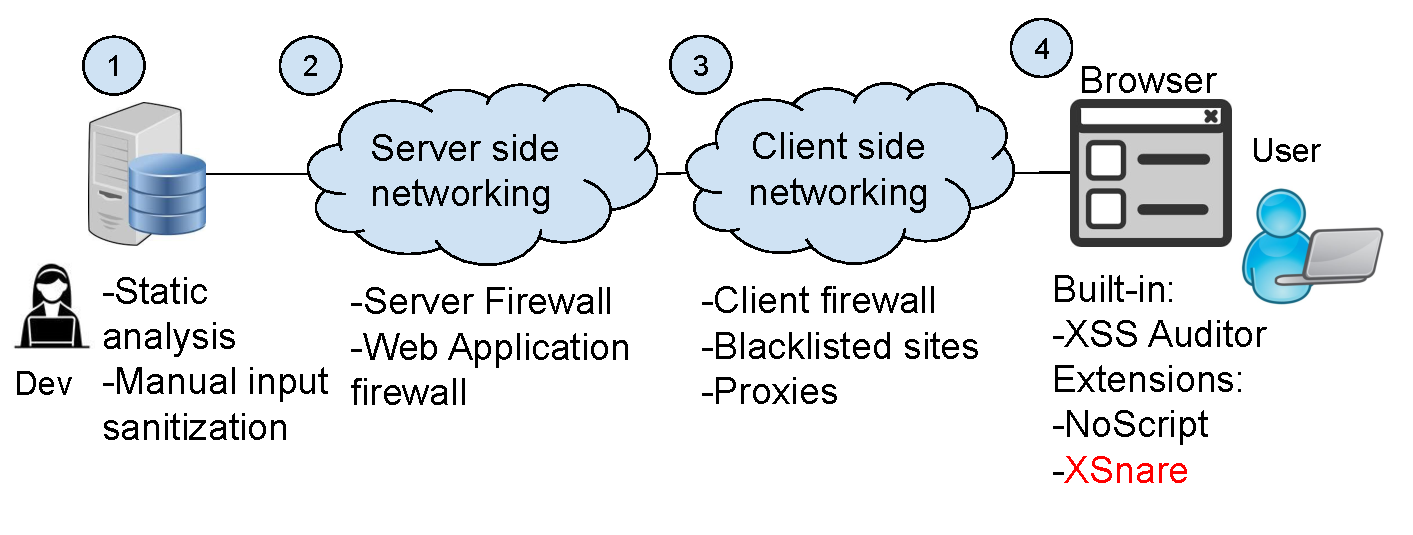
\includegraphics[scale=0.37]{img/web_app_architecture_one.pdf}
  \vspace*{-5.0ex}
%  \caption{Architecture of typical web applications. Different security solutions apply at distinct layers.}
  \caption{Different web security solutions with XSnare on the client-side.}
  \label{fig:web_architecture}
\end{figure}

Vulnerability defences can be implemented in multiple layers of the web application stack (Figure~\ref{fig:web_architecture}). Each layer opens different defence options:
%Further details of these different approaches are described in Section 5:
\begin{enumerate}
	\item At the application's server-side, the developer is
          trying to defend herself against malicious users. The first
          line of defence from these vulnerabilities lies in the
          application logic itself. The developer might choose to
          ensure safety of the code, either by using third-party
          solutions, or by securing the code themselves, for example,
          by applying static analysis on the server code to detect
          unsanitised input.
	\item In the hosting environment, developers deploy
          defences including generic firewalls and more specific \acp{WAF}, which defend against attacks
          such as \ac{DDoS}, \ac{SQL} injections and \ac{XSS}.
	\item In the client's environment, the user requires protection from
          malicious websites, and may install their own network firewall,
          network filters, and web proxies.
	\item The last line of defence is the browser. \sys operates at this point.
          The browser has built-in defences, such as
          Chrome's \ac{XSS} Auditor~\cite{xssauditor}. But the user can also
          install third-party extensions to block malicious requests and
          responses. % such as the NoScript~\cite{Noscript} extension.
\end{enumerate}

Many of these approaches are either unfit for widespread deployment or
do not benefit from an application's contextual knowledge. For
example, a \ac{WAF} might be enough to defend against most \ac{XSS} attacks on
one deployment, but it would require each individual developer to have
the necessary knowledge and resources to integrate one. A network
proxy at the client-side will usually have a generic set of rules to
apply on incoming network traffic, and this will often lead to an
elevated rate of false positives (FPs). Browser built-in defences are very
coarse, and will only work on a subset of exploits. Chrome's XSS
Auditor, for example, only attempts to defend against reflected
\ac{XSS}. Google recently announced its intention to deprecate
XSS Auditor; the reasons include \emph{``Bypasses abound''}, \emph{``It prevents
some legit sites from working''}, and \emph{``Once detected, there's nothing
good to do''}~\cite{deprecatexssauditor}. Stock et
al.~\cite{precise_dom_xss} propose enhancements to 
XSS Auditor and cover a wider range of exploits than the
auditor, but are limited to DOM-based \ac{XSS}. Our work is not particular
to a type of \ac{XSS}.

While there is much work on the server-side~\cite{Xu:2006:TPE:1267336.1267345,DBLP:conf/sec/Nguyen-TuongGGSE05,Pietraszek:2005:DAI:2146257.2146267,Bisht:2008:XPD:1428322.1428325}, the
adoption of server-side techniques might not be feasible for many
developers. A 2018 study found that the average time to patch a \ac{CVE}
regardless of severity is 38 days, increasing to as much as 54 days
for low severity vulnerabilities, and the oldest unpatched \ac{CVE} was 340
days old~\cite{Rapid7}. A client-side solution does not rely on
application developers, so it reduces the turnaround time
between a vulnerability and its patch.
%% IB: Cut for space.
%%
%% Furthermore, it is
%% complementary to the aforementioned techniques: a \ac{WAF} will not reduce
%% the security of a client-side approach, and having these
%% two work in tandem is beneficial to the user's experience.

Furthermore, these defences often do not protect against pure
client-side \ac{XSS}, such as reflected \ac{XSS}, or persistent
client-side \ac{XSS}, which use a browser's local storage or cookies
as an attack vector. Steffens et
al.~\cite{DBLP:conf/ndss/SteffensRJS19} present a study of Persistent
Client-Side \ac{XSS} across popular websites and find that as many as
21\% of the most frequented web sites are vulnerable to these attacks.
%% While some of these exploits are harder to carry out in practice, as
%% many as 6\% of these sites are vulnerable to an attack by a realistic
%% attacker.
%
\textbf{To provide users with the means to protect themselves in the absence
of control over servers, we strongly believe that a novel client-side
solution is necessary.}

A number of existing solutions in this area also suffer from high
rates of false-positives and false-negatives. %% , due to the lack of
%% information available at the layers they operate at.
For example, NoScript~\cite{Noscript} works via domain white-listing, thus by
default, JavaScript scripts and other code will not execute. However,
not all scripts outside of the whitelist should be assumed to be
malicious. Browser-level filters like XSS Auditor work based on
general policies and can therefore incorrectly sanitize non-malicious
content.

\textbf{We posit that the DOM is the right place to mitigate XSS
  attacks as it provides a full picture of the web application.} While
most of the functionality we provide could be done by a network filter
on top of the browser, we require some additional context. In
particular, when an exploit manifests itself through dynamic
behaviour, like a network request initiated by an user's click, we
require knowledge of the tab which initiated the request to filter the
response. Previous work on client-side solutions has focused on
generic approaches to vulnerability
detection~\cite{Kirda:2009:CCS:2639535.2639808,Jim:2007:DSI:1242572.1242654,Hallaraker:2005:DMJ:1078029.1078861}. Our
work is application-specific and can therefore be more precise when
targeting vulnerabilities.

Commonly, bug bounty hunters and penetration testers will scour
websites to find vulnerabilities and alert developers of issues 
and potential fixes. Developers will then fix the bugs
accordingly so that users are not subject to vulnerabilities. Inspired
by this workflow, we believe this process can be partly automated
using a firewall-based approach, so that users do not have to wait for
developers to update their code. A similar approach is presented in~\cite{Kirda:2009:CCS:2639535.2639808}, as a client-side firewall-based 
network proxy. %%  Rules dictate the links which can be accessed by a website
%% when generating requests, and can be created both automatically and manually
%% by a user. 
Unlike our work, this technique does not protect against
attacks which do not generate a network request, such as deleting local
files. 
%% IB: Cut details below -- too detailed.
%% 
%% Furthermore, they rely on websites having a small number of external
%% dynamic links to third-parties. This likely does not hold true anymore, 
%% as websites require an ever-increasing amount of dynamic content, with 
%% several interconnections with third-parties to provide features like advertisements and analytics.



%% IB: Cut the paragraph below -- too technical for intro
%%
%% XSnare consists of three components: a trusted Firefox
%% extension for interposing between the application and the DOM, a
%% periodically updated local database which maintains exploit
%% definitions and descriptions of the vulnerabilities to be targeted by
%% the extension in the form of signatures, and finally, a declarative
%% language for describing exploits, expressive enough for an user to be
%% precise about which parts of the HTML are vulnerable and how to
%% sanitize them.

We aim to reproduce the developer's intended server-side patch on the
client-side, therefore, we need to be able to determine the separation
between dynamic content and the static template, and pass the dynamic
elements to a sanitization function. We further detail XSnare's
mechanisms that achieve this in Section~\ref{xsnare_design}.

We evaluate our application-specific, signature-based approach, by
testing it against recent \ac{XSS} CVEs. CVE databases are
well-maintained and widely available. They are one of the main tools
used by developers to patch their code against known
vulnerabilities. Furthermore, we evaluate the performance overhead of
our extension on web page load times, and show that it does not
significantly affect a user's browsing experience.

In summary, our contributions include: 
\begin{itemize}

	\item XSnare: a novel client-side framework that protects
          users against XSS vulnerabilities with a database of robust
          signatures for these vulnerabilities, written in a
          declarative language.

	\item A mechanism to correctly isolate a vulnerable injection
          point in a web page and to apply the intended server-side
          patch on the client-side.

	\item Evaluation of the efficacy of our protection mechanism
          with a number of XSS CVEs (\autoref{viability}); as well as
          the performance impact of the XSnare browser extension
          (\autoref{performance}). %% , demonstrating that our tool's
          %% feasibility in practice.

\end{itemize}
